\documentclass[a4paper,12pt,twoside]{memoir}

% Castellano
\usepackage[spanish,es-tabla]{babel}
\selectlanguage{spanish}
\usepackage[utf8]{inputenc}
\usepackage[T1]{fontenc}
\usepackage{lmodern} % scalable font
\usepackage{microtype}
\usepackage{placeins}

\RequirePackage{booktabs}
\RequirePackage[table]{xcolor}
\RequirePackage{xtab}
\RequirePackage{multirow}

% Links
\PassOptionsToPackage{hyphens}{url}\usepackage[colorlinks]{hyperref}
\hypersetup{
	allcolors = {red}
}

% Ecuaciones
\usepackage{amsmath}

% Rutas de fichero / paquete
\newcommand{\ruta}[1]{{\sffamily #1}}

% Párrafos
\nonzeroparskip

% Huérfanas y viudas
\widowpenalty100000
\clubpenalty100000

% Evitar solapes en el header
\nouppercaseheads

% Imagenes
\usepackage{graphicx}
\newcommand{\imagen}[2]{
	\begin{figure}[!h]
		\centering
		\includegraphics[width=0.9\textwidth]{#1}
		\caption{#2}\label{fig:#1}
	\end{figure}
	\FloatBarrier
}

\newcommand{\imagenflotante}[2]{
	\begin{figure}%[!h]
		\centering
		\includegraphics[width=0.9\textwidth]{#1}
		\caption{#2}\label{fig:#1}
	\end{figure}
}



% El comando \figura nos permite insertar figuras comodamente, y utilizando
% siempre el mismo formato. Los parametros son:
% 1 -> Porcentaje del ancho de página que ocupará la figura (de 0 a 1)
% 2 --> Fichero de la imagen
% 3 --> Texto a pie de imagen
% 4 --> Etiqueta (label) para referencias
% 5 --> Opciones que queramos pasarle al \includegraphics
% 6 --> Opciones de posicionamiento a pasarle a \begin{figure}
\newcommand{\figuraConPosicion}[6]{%
  \setlength{\anchoFloat}{#1\textwidth}%
  \addtolength{\anchoFloat}{-4\fboxsep}%
  \setlength{\anchoFigura}{\anchoFloat}%
  \begin{figure}[#6]
    \begin{center}%
      \Ovalbox{%
        \begin{minipage}{\anchoFloat}%
          \begin{center}%
            \includegraphics[width=\anchoFigura,#5]{#2}%
            \caption{#3}%
            \label{#4}%
          \end{center}%
        \end{minipage}
      }%
    \end{center}%
  \end{figure}%
}

%
% Comando para incluir imágenes en formato apaisado (sin marco).
\newcommand{\figuraApaisadaSinMarco}[5]{%
  \begin{figure}%
    \begin{center}%
    \includegraphics[angle=90,height=#1\textheight,#5]{#2}%
    \caption{#3}%
    \label{#4}%
    \end{center}%
  \end{figure}%
}
% Para las tablas
\newcommand{\otoprule}{\midrule [\heavyrulewidth]}
%
% Nuevo comando para tablas pequeñas (menos de una página).
\newcommand{\tablaSmall}[5]{%
 \begin{table}
  \begin{center}
   \rowcolors {2}{gray!35}{}
   \begin{tabular}{#2}
    \toprule
    #4
    \otoprule
    #5
    \bottomrule
   \end{tabular}
   \caption{#1}
   \label{tabla:#3}
  \end{center}
 \end{table}
}

%
%Para el float H de tablaSmallSinColores
\usepackage{float}

%
% Nuevo comando para tablas pequeñas (menos de una página).
\newcommand{\tablaSmallSinColores}[5]{%
 \begin{table}[H]
  \begin{center}
   \begin{tabular}{#2}
    \toprule
    #4
    \otoprule
    #5
    \bottomrule
   \end{tabular}
   \caption{#1}
   \label{tabla:#3}
  \end{center}
 \end{table}
}

\newcommand{\tablaApaisadaSmall}[5]{%
\begin{landscape}
  \begin{table}
   \begin{center}
    \rowcolors {2}{gray!35}{}
    \begin{tabular}{#2}
     \toprule
     #4
     \otoprule
     #5
     \bottomrule
    \end{tabular}
    \caption{#1}
    \label{tabla:#3}
   \end{center}
  \end{table}
\end{landscape}
}

%
% Nuevo comando para tablas grandes con cabecera y filas alternas coloreadas en gris.
\newcommand{\tabla}[6]{%
  \begin{center}
    \tablefirsthead{
      \toprule
      #5
      \otoprule
    }
    \tablehead{
      \multicolumn{#3}{l}{\small\sl continúa desde la página anterior}\\
      \toprule
      #5
      \otoprule
    }
    \tabletail{
      \hline
      \multicolumn{#3}{r}{\small\sl continúa en la página siguiente}\\
    }
    \tablelasttail{
      \hline
    }
    \bottomcaption{#1}
    \rowcolors {2}{gray!35}{}
    \begin{xtabular}{#2}
      #6
      \bottomrule
    \end{xtabular}
    \label{tabla:#4}
  \end{center}
}

%
% Nuevo comando para tablas grandes con cabecera.
\newcommand{\tablaSinColores}[6]{%
  \begin{center}
    \tablefirsthead{
      \toprule
      #5
      \otoprule
    }
    \tablehead{
      \multicolumn{#3}{l}{\small\sl continúa desde la página anterior}\\
      \toprule
      #5
      \otoprule
    }
    \tabletail{
      \hline
      \multicolumn{#3}{r}{\small\sl continúa en la página siguiente}\\
    }
    \tablelasttail{
      \hline
    }
    \bottomcaption{#1}
    \begin{xtabular}{#2}
      #6
      \bottomrule
    \end{xtabular}
    \label{tabla:#4}
  \end{center}
}

%
% Nuevo comando para tablas grandes sin cabecera.
\newcommand{\tablaSinCabecera}[5]{%
  \begin{center}
    \tablefirsthead{
      \toprule
    }
    \tablehead{
      \multicolumn{#3}{l}{\small\sl continúa desde la página anterior}\\
      \hline
    }
    \tabletail{
      \hline
      \multicolumn{#3}{r}{\small\sl continúa en la página siguiente}\\
    }
    \tablelasttail{
      \hline
    }
    \bottomcaption{#1}
  \begin{xtabular}{#2}
    #5
   \bottomrule
  \end{xtabular}
  \label{tabla:#4}
  \end{center}
}



\definecolor{cgoLight}{HTML}{EEEEEE}
\definecolor{cgoExtralight}{HTML}{FFFFFF}

%
% Nuevo comando para tablas grandes sin cabecera.
\newcommand{\tablaSinCabeceraConBandas}[5]{%
  \begin{center}
    \tablefirsthead{
      \toprule
    }
    \tablehead{
      \multicolumn{#3}{l}{\small\sl continúa desde la página anterior}\\
      \hline
    }
    \tabletail{
      \hline
      \multicolumn{#3}{r}{\small\sl continúa en la página siguiente}\\
    }
    \tablelasttail{
      \hline
    }
    \bottomcaption{#1}
    \rowcolors[]{1}{cgoExtralight}{cgoLight}

  \begin{xtabular}{#2}
    #5
   \bottomrule
  \end{xtabular}
  \label{tabla:#4}
  \end{center}
}




\graphicspath{ {./img/} }

% Capítulos
\chapterstyle{bianchi}
\newcommand{\capitulo}[2]{
	\setcounter{chapter}{#1}
	\setcounter{section}{0}
	\setcounter{figure}{0}
	\setcounter{table}{0}
	\chapter*{#2}
	\addcontentsline{toc}{chapter}{#2}
	\markboth{#2}{#2}
}

% Apéndices
\renewcommand{\appendixname}{Apéndice}
\renewcommand*\cftappendixname{\appendixname}

\newcommand{\apendice}[1]{
	%\renewcommand{\thechapter}{A}
	\chapter{#1}
}

\renewcommand*\cftappendixname{\appendixname\ }

% Formato de portada
\makeatletter
\usepackage{xcolor}
\newcommand{\tutor}[1]{\def\@tutor{#1}}
\newcommand{\course}[1]{\def\@course{#1}}
\definecolor{cpardoBox}{HTML}{E6E6FF}
\def\maketitle{
  \null
  \thispagestyle{empty}
  % Cabecera ----------------
\noindent
\includegraphics[width=\textwidth]{cabecera}\vspace{1cm}%
  \vfill
  % Título proyecto y escudo informática ----------------
  \colorbox{cpardoBox}{%
    \begin{minipage}{.8\textwidth}
      \vspace{.5cm}\Large
      \begin{center}
      \textbf{TFG del Grado en Ingeniería Informática}\vspace{.6cm}\\
      \textbf{\LARGE\@title{}}
      \end{center}
      \vspace{.2cm}
    \end{minipage}

  }%
  \hfill\begin{minipage}{.20\textwidth}
    
\includegraphics[width=\textwidth]{escudoInfor}
  \end{minipage}
  \vfill
  % Datos de alumno, curso y tutores ------------------
  \begin{center}%
  {%
    \noindent\LARGE
    Presentado por \@author{}\\ 
    en Universidad de Burgos --- \@date{}\\
    Tutores: \@tutor{}\\
  }%
  \end{center}%
  \null
  \cleardoublepage
  }
\makeatother


% Datos de portada
\title{X-Teeth \\Documentación Técnica}
\author{Ismael Franco Hernando}
\tutor{César Ignacio García Osorio y\\ José Miguel Ramírez Sanz}
\date{\today}

\begin{document}

\maketitle



\cleardoublepage



%%%%%%%%%%%%%%%%%%%%%%%%%%%%%%%%%%%%%%%%%%%%%%%%%%%%%%%%%%%%%%%%%%%%%%%%%%%%%%%%%%%%%%%%



\frontmatter


\clearpage

% Indices
\tableofcontents

\clearpage

\listoffigures

\clearpage

\listoftables

\clearpage

\mainmatter

\appendix

\apendice{Plan de Proyecto Software}

\section{Introducción}
Dentro de este apartado se van a tratar dos puntos acerca del proyecto:
\begin{itemize}
    \item La Planificación temporal.
    \item La Viabilidad del mismo.
\end{itemize}
\section{Planificación temporal}
Para llevar a cabo el proyecto se ha seguido la metodología de trabajo \emph{Scrum}, dónde cada semana se llevaba a cabo un \emph{sprint} distinto. En cada uno de estos \emph{sprints} se consensuaban unos objetivos y tareas a llevar a cabo para la siguiente semana.

En situaciones especiales, las reuniones se podrían atrasar unas semanas con el fin de desempeñar correctamente los objetivos marcados.

Para poder reflejar el trabajo que se iba realizando semana tras semana se utilizó la plataforma de \emph{GitHub} cuyo repositorio que recoge el trabajo del proyecto es \url{https://github.com/ifh1001/TFG_X-Teeth}.

\subsection{Sprint 1 - 02/02/2022}
Este primer \emph{sprint} se basó principalmente en la explicación por parte de mis tutores sobre el trabajo a realizar en el TFG X-Teeth. Además, se concretó la fecha de las reuniones de cada \emph{sprint}, siendo esta los viernes a las 11:30 de la mañana a través de \emph{Microsoft Teams}.

Como primeras tareas a llevar a cabo fueron:
\begin{itemize}
    \item Crear cuenta en \emph{Overleaf}, para hacer la documentación con \LaTeX.
    \item Crear el repositorio en \emph{GitHub}.
    \item Leer diversos artículos sobre el \emph{Deep Learning} en la rama de la odontología.
    \item Buscar información acerca de la librería de \emph{Keras}, ya que se pensó que podría ser una solución para llevar a cabo el proyecto.
\end{itemize}
\subsection{Sprint 2 - 11/02/2022}
En esta segunda reunión se habló sobre los pocos casos de dientes que había para poder trabajar y que mi tutor José Miguel había estado desarrollando un \emph{notebook} que hacía uso del \emph{data augmentation} para así disponer de un mayor número de casos distintos. 

También, debido al problema de tener pocas radiografías, se decidió usar \emph{Detectron2}, ya que es una biblioteca de \emph{Python} que permite detectar objetos con muy pocos casos.
Como resultado de esta reunión, las tareas a desarrollar para la siguiente semana fueron:
\begin{itemize}
    \item Terminar el \emph{notebook} de mi tutor.
    \item Intentar instalar \emph{Detectron2} en mi ordenador.
\end{itemize}

\subsection{Sprint 3 - 18/02/2022}
Para este \emph{sprint} solo puede terminar el \emph{notebook}, ya que la parte de instalación de \emph{Detectron2} me resultó imposible, debido a que no existe una versión oficial para trabajar con Windows 10 y generalmente surgen incompatibilidades entre varios paquetes en este sistema operativo. Como resultado de esto, la única tarea a realizar para el siguiente \emph{sprint} fue seguir intentando instalar \emph{Detectron2}.

\subsection{Sprint 4 - 23/02/2022}
Esta reunión fue distinta a las anteriores, ya que inicialmente mantuvimos una charla con el odontólogo que da origen a este proyecto. Se le comentó que había un error en algunos de los casos que nos había pasado y se acordó que nos pasaría un total de 150 radiografías para poder trabajar correctamente con \emph{Detectron2}.

La segunda parte de la reunión fue ya sin el odontólogo, en la cual comenté que no conseguí instalar \emph{Detectron2}. Debido a esta situación, se decidió trabajar por el momento con \emph{Google Colab}, ya que era muy sencillo usar la librería de detección de objetos, y en el futuro utilizar alguna de las máquinas a disposición de la Universidad de Burgos, como Gamma o Beta. 

Las tareas resultantes este \emph{sprint} fueron:
\begin{itemize}
    \item Aprender a utilizar \emph{Detectron2} en \emph{Google Colab}.
    \item Crear una función que transformara los archivos JSON del dentista a la forma COCO que necesita \emph{Detectron2} para poder trabajar.
\end{itemize}

\subsection{Sprint 5 - 04/03/2022}
Para este \emph{sprint} tras haber realizado con éxito la segunda tarea de la reunión pasada, creé el primer sistema entrenador de \emph{Detectron2}, dónde, pese a trabajar con tan solo 10 imágenes (7 para entrenar y 3 para testear) se obtuvieron unos resultados bastante buenos en la parte de detección del diente y regulares en la parte del nervio.

Tras obtener estos resultados tan esperanzadores, las siguientes tareas a hacer fueron:
\begin{itemize}
    \item Aplicar la técnica \emph{Convex Hull} a las imágenes rotadas obtenidas por el \emph{notebook} terminado del  \emph{sprint} 2, con el fin de obtener los puntos de la máscara y generar los JSON correspondientes y poder trabajar con más casos.
    \item Aplicar la técnica IoU (\emph{Intersection over Union}), para comprobar si las predicciones del \emph{Detectron2} están siendo buenas.
\end{itemize}

\subsection{Sprint 6 - 11/03/2022}
Los resultados obtenidos por el \emph{Convex Hull} no fueron los correctos, ya que esta técnica no funciona correctamente en las zonas curvas de los dientes y nervios.

Además, detecte un problema en el \emph{notebook} del \emph{sprint} 2, puesto que las máscaras de los dientes y nervios no se encontraban en el tamaño correcto con respecto a la imagen de la radiografía correspondiente.

Por último, se creyó conveniente aplicar otra estrategia con el \emph{Detectron2}, ya que inicialmente teníamos un modelo para entrenar a la vez dientes y nervios, por lo que se pensó que con la siguiente estrategia se conseguirían mejores resultados:
\begin{enumerate}
    \item Crear un modelo que solo entrenara dientes.
    \item Obtener las predicciones de los dientes.
    \item Recortar la caja que contenía el diente de la predicción.
    \item Crear un modelo que únicamente entrenara nervios.
    \item Obtener las predicciones de los nervios.
\end{enumerate}
Por tanto, para el siguiente \emph{sprint} tendría que realizar las siguientes tareas:
\begin{itemize}
    \item Buscar una técnica que realice correctamente la detección de los puntos de las máscaras de los dientes y nervios.
    \item Solucionar el problema de tamaños entre las máscaras y la radiografía.
    \item Llevar a cabo la nueva estrategia del \emph{Detectron2}.
    \item Mostrar una gráfica con la \emph{pérdida total} durante el entrenamiento con el fin de ver a partir de que iteración se produce un \emph{overfitting}.
\end{itemize}

\subsection{Sprint 7 - 25/03/2022}
En el anterior \emph{sprint} se completaron con éxito todas las tareas. Pese a ello, la técnica aplicada para detectar los bordes gracias a la librería CV2 de \emph{Python} obtuvo unos buenos resultados aunque no del todo precisos.

Por tanto, sería útil buscar alguna otra alternativa con el fin de ver si se puede conseguir una mayor precisión en la detección de los puntos de los bordes de las máscaras.

Como resultado de esta reunión, las tareas a realizar para la siguiente semana son:
\begin{itemize}
    \item Buscar alguna alternativa en la detección de bordes, con el fin de conseguir mejores resultados.
    \item Entrenar \emph{Detectron2} con las radiografías originales y no con las que tienen el diente resaltado, ya que seguramente se estén consiguiendo buenos resultados gracias a la ``ayuda'' que dispone en las imágenes.
    \item Buscar información acerca de la convención PEP8, y empezar a aplicarlo, con el fin de conseguir un código más limpio.
    \item Añadir un límite en la parte de validación para que una vez se encuentre el punto en el que se produce el \emph{overfitting} no siga entrenando.  
\end{itemize}

\subsection{Sprint 8 - 01/04/2022}
En esta semana se ha conseguido mejorar la forma de obtener los puntos de las máscaras de los dientes y nervios, para poder trabajar correctamente con ellas. 

Esto se ha conseguido juntando dos librerías: inicialmente se usa \emph{scikit-image} para obtener únicamente el borde de cada una de las máscaras y, a continuación, se utiliza CV2 para conseguir todos los puntos que dan lugar a ese borde. De esta manera se consigue una precisión mucho mayor que aplicando únicamente CV2 sobre las imágenes.

Las próximas tareas a realizar son:
\begin{itemize}
    \item Instalar \emph{Detectron2} en la máquina de la Universidad de Burgos, Gamma, para poder trabajar en ella.
    \item Automatizar el proceso de repartición del conjunto de datos de modo que el 60\% sea de entrenamiento, un 20\% para test y el último 20\% para validación. 
\end{itemize}

\subsection{Sprint 9 - 22/04/2022}
Para este \emph{sprint} no se consiguió instalar \emph{Detectron2} en la máquina Gamma debido a alguna incompatibilidad entre versiones. Pese a ello, se siguió trabajando en \emph{Google Colab}, y se crearon las funciones necesarias para poder distribuir las imágenes de manera aleatoria entre el entrenamiento, validación y test. 

Adicionalmente, se añadió de forma correcta el cálculo de la precisión de las predicciones a través del IoU ya mencionado anteriormente. Dicho valor se calculó tanto en el \emph{notebook} de dos modelos entrenadores cómo en el de un modelo entrenador, con el fin de ver cuál de ellos muestra mejores resultados, que por el momento es el segundo.

Por último, se mejoró el código en uno de los \emph{notebook} para facilitar la comprensión del mismo a través del estándar PEP8.

La tarea a realizar para la próxima semana es:
\begin{itemize}
    \item Conseguir instalar \emph{Detectron2} en Gamma mediante versiones más antiguas de los paquetes con el fin de evitar incompatibilidades.
\end{itemize}

\subsection{Sprint 10 - 29/04/2022}
Para esta semana se ha conseguido instalar \emph{Detectron2} en Gamma. Para ello, se han tenido que utilizar versiones antiguas tanto de \emph{CUDA Toolkit} cómo de  \emph{PyTorch} para poder evitar las distintas incompatibilidades entre versiones.

Se han instalado la versión 10.1 de \emph{CUDA Toolkit} y la versión 1.4 de \emph{PyTorch}, junto con la versión del \emph{Detectron2} compatible para soportar dichas librerías.

Las dos tareas próximas a realizar son:
\begin{itemize}
    \item Implementar de forma correcta el método para poder medir el tamaño del nervio del diente de la imagen.
    \item Investigar las distintas GUI de \emph{Python} para elegir una de ellas y poder montar la aplicación final.  
\end{itemize}

\subsection{Sprint 11 - 06/05/2022}
Para este \emph{sprint} se ha implementado una técnica que permite calcular la longitud del nervio. Dicha técnica se basa en obtener la distancia máxima entre el nervio y el diente. Pese a que se ha conseguido que funcione correctamente, estamos a la espera del dentista para poder transformar la distancia en píxeles a una longitud real y poder analizar los resultados que da.

La segunda técnica que se quería implementar se basaba en usar \emph{Skeletonize} de la librería \emph{scikit-image}. Dicha técnica no se ha implementado de forma correcta y, por tanto, aún no se sabe si puede dar buenos resultados.

Con respecto a las GUI de \emph{Python}, tras analizar varias se ha decidido trabajar con \emph{EasyGUI} y con \emph{PySimpleGUI}. Y una vez se hayan probado ambas elegir una de las dos.

Como resultado, las tareas a realizar para la semana que viene son:
\begin{itemize}
    \item Corregir el uso de \emph{Skeletonize} para que funcione correctamente y ver que resultados da.
    \item Instalar \emph{EasyGui} y \emph{PySimpleGui} en el entorno de \emph{conda} de Gamma para ver que funcionen correctamente y seleccionar la mejor.
\end{itemize}

\subsection{Sprint 12 - 13/05/2022}
Para esta reunión han ocurrido dos hechos importantes. El primero es que a mitad del \emph{sprint} anterior el odontólogo que da origen a este proyecto había cambiado de idea. Inicialmente, lo principal era obtener la medida del nervio, pero ahora el odontólogo quiere la longitud del diente.

El segundo hecho relevante, ha sido que el propio odontólogo ha asistido a la reunión para ver los resultados que se están consiguiendo. También, nos comentó el proceso que realiza para poder medir el tamaño del diente y al mostrarle las técnicas que utilizamos para calcular la longitud nos indicó que la correcta sería la que mide el diente por los puntos centrales.

Como última cosa a comentar sería la imposibilidad de poder ejecutar un GUI desde el \emph{notebook} en Gamma, debido a que al ser un servidor no tiene ningún \emph{display}
asignado. Por ello, la aplicación final se llevará a cabo en un \emph{notebook}.

Las próximas tareas a hacer son:
\begin{itemize}
    \item Investigar y probar \emph{ipywidgets} con el fin de poder tener una pequeña interfaz dentro del \emph{notebook} que contendrá la aplicación final.
    \item Para poder medir la longitud del diente por la parte central, se ha pensado en emplear \emph{Skeletonize} sobre el nervio y a la lineal central obtenida alargarla hasta el diente, para posteriormente calcular su longitud.
\end{itemize}

\subsection{Sprint 13 - 20/05/2022}
Para este \emph{sprint} se ha implementado la técnica para medir la longitud del diente a través de la línea central del nervio. Con dicha técnica se han implementado un total de tres técnicas distintas para poder calcular el tamaño del diente.

Pese a tener varias técnicas, ninguna de ellas parece que da buenos resultados por el momento, ya que los errores relativos son demasiados altos para que el odontólogo pueda usar algunos de estos métodos.

Con respecto a \emph{ipywidgets}, se ha conseguido instalar, además de investigar y probar los distintos tipos de \emph{widgets} que hay con el fin de ver cuáles utilizar en la aplicación final.

Las tareas a realizar para la próxima semana son:
\begin{itemize}
    \item Investigar porque los resultados obtenidos no son los esperados, ya que el proceso de segmentación es bastante bueno.
    \item Desarrollar la aplicación final con las distintas funcionalidades de \emph{ipywidgets}.
\end{itemize}

\subsection{Sprint 14 - 27/05/2022}
Para esta semana se ha conseguido desarrollar una simple aplicación que permita subir al odontólogo una radiografía y que le presente los resultados obtenidos. Actualmente, la aplicación muestra la radiografía junto con la recta correspondiente a la longitud del diente y un cuadro de texto con el tamaño del mismo.

Con respecto a los errores que se estaban obteniendo a la hora de calcular la longitud de los dientes, tras analizar los métodos implementados y la segmentación de dientes y nervios por parte de \emph{Detectron2}, se ha llegado a la conclusión de que el problema probablemente venga dado o por la resolución que nos pasó el odontólogo o por los tamaños de los dientes que nos indicó en las distintas radiografías.

Para la siguiente semana las tareas a realizar son:
\begin{itemize}
    \item Permitir subir en la aplicación varias radiografías a la vez y mostrar para cada una de ellas los resultados obtenidos.
    \item En la aplicación, mostrar la segmentación del diente y el nervio obtenida en cada caso.
    \item Probar a exportar el modelo obtenido del \emph{Detectron2} a un \emph{notebook} en \emph{Google Colab} con el fin de facilitar las conexiones a la aplicación.
    \item En caso de que la tarea anterior no se pueda efectuar, usar \emph{tmux} junto con \emph{Ngrok} para permitir conexiones al \emph{notebook} que tiene la aplicación en Gamma.
\end{itemize}

\subsection{Sprint 15 - 03/06/2022}
Para esa semana se han conseguido implementar las distintas mejoras de la aplicación final. 

Con respecto al modelo, al ser un archivo pesado de unos 330 MB aproximadamente, hay problemas a la hora de subirlo tanto a \emph{Google Colab} como a \emph{GitHub}. Por ello, no se ha podido probar si el modelo funcionará en la aplicación subida a \emph{Google Colab}.

Por último, mencionar que el dentista nos ha indicado que la última técnica que usamos para medir la longitud de los dientes no es la correcta en aquellos casos donde el nervio tenga una cierta curvatura. Por tanto, hay que implementar una cuarta técnica que mida la longitud del diente a través del nervio, calculando las longitudes en pequeñas porciones para poder medir correctamente las zonas curvas de los dientes.

Las próximas tareas a realizar son:
\begin{itemize}
    \item Buscar si existe algún \emph{widget} que permita hacer zum a las imágenes, para poder observar mejor los resultados obtenidos en la aplicación.
    \item Con el fin de dar más \emph{feedback} al usuario en la aplicación a la hora de cargar las imágenes, mostrar un mensaje con las distintas imágenes cargadas.
    \item Usar alguna técnica que permita dividir el modelo en pequeños archivos para poder trabajar con ello de forma cómoda.
    \item Implementar la nueva técnica de cálculo de longitud del diente mencionada anteriormente.
\end{itemize}

\subsection{Sprint 16 - 10/06/2022}
Para este \emph{sprint} se ha buscado algún \emph{widget} que permita hacer zum a las imágenes en los resultados de la aplicación, pero no se ha encontrado nada útil. También, se ha añadido que cada vez que se cargue una imagen se muestre un mensaje con el nombre de todas las imágenes cargadas.

Con respecto a la técnica a implementar, se ha desarrollado correctamente. Pero la parte de buscar la distancia máxima desde el extremo del nervio hasta el diente no es la correcta, por lo que se realizará de igual forma que la técnica anterior, alargar como si fuera una línea recta hasta el borde del diente.

Por otro lado, con respecto a dividir el modelo para poder subirlo a \emph{Google Colab} y a \emph{GitHub}, se ha encontrado una forma más sencilla. Dicho modo se basa en tener el modelo subido en \emph{Google Drive} y gracias al paquete \emph{gdown} descargarlo.

Tras poder subirlo a \emph{Google Colab}, se ha corroborado que se puede utilizar el modelo obtenido en Gamma en los \emph{notebooks} de \emph{Google}.

Por último, la aplicación en Gamma se ha lanzado también con \emph{Ngrok}, de manera que, actualmente, se puede acceder a la aplicación a través de un enlace. Pese a ello, también se va a realizar la aplicación en \emph{Google Colab}, de modo que haya dos alternativas para poder usarla.

Por tanto, las tareas a hacer para la semana que viene son:
\begin{itemize}
    \item Corregir el problema de la cuarta técnica implementada para calcular la longitud del diente.
    \item Una vez esté corregido el problema de la tarea anterior, actualizar la aplicación para que trabaje con dicha estrategia para calcular la longitud deseada.
    \item Implementar la aplicación en \emph{Google Colab}.
    \item Comentar las diversas celdas de los diferentes \emph{notebooks} para facilitar su comprensión. 
\end{itemize}

\subsection{Sprint 17 - 16/06/2022}
Para esta semana se ha solucionado el problema de la última técnica implementada. También se ha actualizado la aplicación para que trabaje con dicha técnica.

La aplicación también se ha desarrollado y probado en \emph{Google Colab}, donde funciona correctamente.

Con respecto a comentar las celdas de todos los \emph{notebooks}, se ha empezado, pero no se ha terminado.

Las próximas tareas a realizar son:
\begin{itemize}
    \item Terminar de comentar todos los \emph{notebooks}.
    \item Retocar la aplicación, añadiendo manual de usuario y más descripciones y efectuando alguna pequeña mejora.
\end{itemize}

\subsection{Sprint 18 - 24/06/2022}
Este fue el último \emph{sprint} del proyecto. En él se revisó la aplicación final y se revisó parte de la documentación que se llevaba hecha. Con respecto a la documentación de los diferentes \emph{notebooks} no se consiguió comentar todos los subidos a lo largo del proyecto a \emph{GitHub}.

Por tanto, las últimas tareas a realizar son:
\begin{itemize}
    \item Terminar de comentar todos los \emph{notebooks}.
    \item Terminar de escribir toda la documentación del proyecto.
\end{itemize}

\section{Estudio de viabilidad}
En los siguientes apartados se procederá a estudiar, tanto la viabilidad económica como la viabilidad legal del proyecto.

\subsection{Viabilidad económica}
Para estimar la viabilidad económica se analizarán dos elementos importantes, primero el coste de mantener al personal de la aplicación y segundo el coste del hardware necesario para tener siempre activa la aplicación.
\subsubsection{Coste del personal}
Para llevar a cabo la aplicación y mantenerla a lo lago del tiempo se va a suponer que se contrata a un programador cuyo sueldo medio en España es de unos 29.800€ brutos al año, lo que supone unos 1.610€ netos al mes (valores obtenidos en Jobted\footnote{ Jobted: \url{https://www.jobted.es/salario/programador}}).

\begin{center}
\begin{tabular}{|c|c|}
\hline
\textbf{Coste estimado por mes} & \numprint{1610}€ \\ \hline
\textbf{Coste estimado año}     & \numprint{19320}€ \\ \hline
\end{tabular}
\captionof{table}{Costes estimados personal}
\end{center}

\subsubsection{Hardware}
La aplicación puede usarse de dos formas distintas:
\begin{itemize}
    \item Gamma: accediendo al \emph{notebook} alojado en la máquina de la Universidad de Burgos.
    \item Google Colab: accediendo al \emph{notebook} compartido de Colab.
\end{itemize}

Debido a las dos opciones que hay para usar la aplicación se podrían distinguir dos costes distintos.

Por un lado tenemos \emph{Google Colab} donde se puede compartir \emph{notebooks} de forma gratuita a otros usuarios a través de un enlace que les da acceso. 

Por el otro lado, tenemos el \emph{notebook} en Gamma, por lo que la máquina tiene que estar siempre activa para no dejar a los clientes sin servicio. Debido a ello, tendrá que encontrase la máquina siempre conectada a la red eléctrica.

\begin{center}
\begin{tabular}{|c|c|}
\hline
\textbf{Coste estimado por mes} & \numprint{100}€  \\ \hline
\textbf{Coste estimado año}     & \numprint{1200}€ \\ \hline
\end{tabular}
\captionof{table}{Costes estimados hardware}
\end{center}

\subsubsection{Costes Totales}
Tras analizar los costes del personal y los costes del hardware, los costes estimado al mes y al año son:
\begin{center}
\begin{tabular}{c|c|c|}
\cline{2-3}
                                              & \textbf{Mes} & \textbf{Año} \\ \hline
\multicolumn{1}{|c|}{\textbf{Coste Personal}} & \numprint{1610}€        & \numprint{19320}€       \\ \hline
\multicolumn{1}{|c|}{\textbf{Coste Hardware}} & \numprint{100}€         & \numprint{1200}€        \\ \hline
\multicolumn{1}{|c|}{\textbf{Total}}          & \numprint{1710}€        & \numprint{20520}€       \\ \hline
\end{tabular}
\captionof{table}{Costes estimados totales}
\end{center}

\subsection{Viabilidad legal}
Con respecto a la viabilidad legal, se han empleado bibliotecas de \emph{Python} que permiten su uso y comercialización gratuita. 

El principal problema viene con las radiografías, ya que nos las ha prestado el odontólogo y por ello no se pueden subir con este proyecto para que puedan probarse. Esto podría suponer un problema, puesto que cualquier usuario que quiera comprobar como funciona la aplicación necesitará poseer alguna radiografía dental.

Incluso para la gente que quiera replicar este proyecto, por su parte, deberá de tener un número razonable de radiografías para poder entrenar su modelo de manera correcta.

Las bibliotecas de \emph{Python} utilizadas en la aplicación final junto con la licencia asociada a cada una de ellas se puede ver en la tabla \ref{licencias}.
\begin{center}
\begin{tabular}{|l|l|}
\hline
\textbf{Biblioteca} & \textbf{Licencia} \\ \hline
NumPY               & BSD               \\ \hline
OpenCV              & BSD               \\ \hline
Matplotlib          & PSF               \\ \hline
Jupyter Widgets     & BSD               \\ \hline
Detectron2          & Apache 2.0        \\ \hline
SciPy               & BSD               \\ \hline
PyTorch             & BSD               \\ \hline
Scikit-Image        & BSD               \\ \hline
gdown               & MIT               \\ \hline
\end{tabular}
\captionof{table}{Licencias Bibliotecas Python}
\label{licencias}
\end{center}

Todas estas licencias, junto con la licencia BSD de \emph{Jupyter Notebook} permiten que la aplicación final pueda ser distribuida y comercializada sin ninguna limitación.

Tras analizar todas las licencias, la licencia colocada al proyecto es GPL v3 que permite la comercialización del \emph{software} desarrollado, su modificación, distribución, realizar patentes y su uso de forma privada.
\apendice{Especificación de Requisitos}

\section{Introducción}

\section{Objetivos generales}

\section{Catalogo de requisitos}

\section{Especificación de requisitos}



\apendice{Especificación de diseño}

\section{Introducción}

\section{Diseño de datos}

\section{Diseño procedimental}

\section{Diseño arquitectónico}



\apendice{Documentación técnica de programación}

\section{Introducción}

\section{Estructura de directorios}

\section{Manual del programador}

\section{Compilación, instalación y ejecución del proyecto}

\section{Pruebas del sistema}

\apendice{Documentación de usuario}

\section{Introducción}
En este apartado se hablará acerca de los diferentes requisitos de usuario, el proceso de instalación para la aplicación del proyecto y el manual de usuario con el fin de que quede explicado cómo usar la aplicación.

\section{Requisitos de usuarios}
Los requisitos de usuario necesarios son muy sencillos, tan solo es necesario que el usuario disponga de una conexión a internet con la que poder conectarse al \emph{notebook} de Gamma o de \emph{Google Colab}.

Como requisito adicional tendrá que conocer el enlace que le permitiría acceder a dichos \emph{notebooks}.

\section{Instalación}
Para poder disfrutar de la aplicación no es necesaria ninguna instalación en el ordenador del usuario. Tan solo será necesario instalar \emph{Detectron2} en el \emph{notebook} de \emph{Google Colab}, ya que no tiene por defecto la librería necesaria y cada sesión será necesaria su instalación al borrar todos los directorios de la aplicación al finalizar la sesión de \emph{Colab}.

De forma contraria, en Gamma se podrá utilizar la aplicación sin instalar ningún paquete adicional, porque la máquina siempre cuenta con todas las librerías necesarias en el entorno instaladas.

\section{Manual del usuario}
Al poder usar la aplicación desde dos métodos distintos, según donde nos encontremos tendremos un manual de usuario u otro.

\subsection{Google Colab}
Una vez hayamos accedido al \emph{notebook} de \emph{Google Colab} es turno de instalar y descargar todo lo necesario antes de poder utilizar la aplicación. Esto se debe principalmente a que \emph{Google} borra todo el contenido al finalizar sesión y no está instalado \emph{Detectron2} por lo que es necesaria su instalación.

Para poder ejecutar las celdas del \emph{notebook} hay que pulsar al botón circular (Figura \ref{f:play}) que se encuentra al lado izquierdo de cada celda.

\begin{figure}[h]
 \centering
  
\includegraphics[width=0.07\textwidth]{img/Play.PNG}
 \caption{Botón Ejecución Google Colab}
 \label{f:play}
\end{figure}

El primer paso será descargar e instalar \emph{Detectron2} que es un proceso que suele tomar unos minutos. A continuación, se descargan las funciones de la aplicación, subidas al repositorio de \emph{GitHub} del proyecto.

Lo siguiente será importar todas las bibliotecas necesarias para el correcto funcionamiento de la aplicación. También será necesario descargarse el modelo de \emph{Google Drive}, que aunque es pesado, tarda apenas unos segundos en descargarse.

Ahora ya se dispone de todo lo necesario para poder usar la aplicación. Es turno de subir las radiografías, para ello se ejecutará la celda \textbf{Cargar Imagen}. Ahora habrá aparecido un botón (Figura \ref{f:upload}) que permite subir las radiografías a la aplicación.

Finalmente, se ejecutará la celda \textbf{Calcular Longitud}. Tras esperar unos segundos empezarán a aparecer los resultados, formados por la radiografía original, la radiografía segmentada (detección del diente y nervio) y la radiografía con la recta por la cual se ha obtenido su longitud. También, aparecerá un recuadro para cada radiografía con su longitud (Figura \ref{apli}).

\begin{figure}[h]
    \centering
    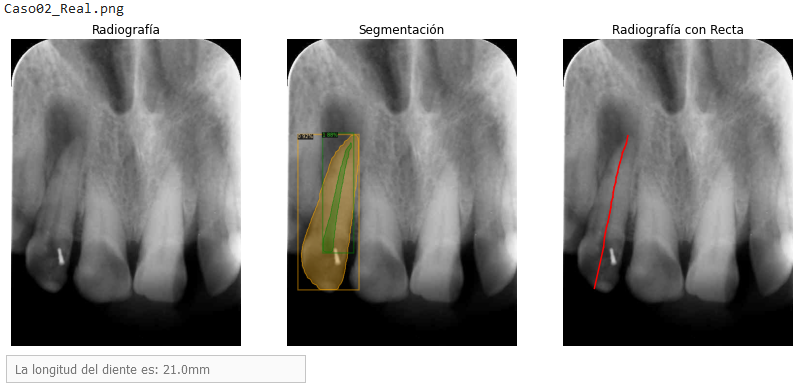
\includegraphics[scale=0.6]{./img/ResultadoApl.png}
    \caption{Resultado Aplicación Final.}
    \label{apli}
\end{figure}

\subsection{Gamma}
Una vez hayamos entrado a \emph{Jupyer Notebook} a través de la herramienta \emph{Ngrok}, hay que dirigirse a la aplicación, que se corresponde al fichero \texttt{Aplicacion.ipynb}.

Una vez nos encontremos en el interior del \emph{notebook} hay que importar todos los paquetes necesarios en la aplicación. Para ello nos colocamos en la primera celda y usaremos el botón del menú superior \textbf{Run}. Una vez se haya terminado de ejecutar, aparecerá a su izquierda el número 1, como se aprecia en la Figura \ref{f:celda1}.

\begin{figure}[h]
 \centering
  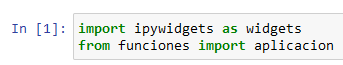
\includegraphics[width=0.6\textwidth]{img/Gamma1.PNG}
 \caption{Ejemplo Ejecución Celda 1 Aplicación}
 \label{f:celda1}
\end{figure}

A continuación, es turno de preparar la subida de las radiografías a la aplicación. Para ello, nos colocamos en la siguiente celda y la ejecutamos de igual manera. Ahora aparecerá un botón, llamado \textbf{Upload} (Figura \ref{f:upload}), que al pulsarlo nos permitirá subir todas las radiografías deseadas.

\begin{figure}[h]
 \centering
  
\includegraphics[width=0.3\textwidth]{img/Gamma2.PNG}
 \caption{Botón Upload}
 \label{f:upload}
\end{figure}

Para poder subir varias radiografías a la vez, es tan sencillo como mantener pulsada la tecla \emph{Ctrl} e ir seleccionando todas las radiografías deseadas.

Una vez se hayan subido las imágenes, aparecerá un mensaje en la celda con los nombres de las radiografías cargadas. Ahora es momento de ejecutar el proceso de cálculo. Para ello, nos vamos a la tercera celda y la ejecutamos. Tras esperar unos segundos empezarán a aparecer los resultados, formados por la radiografía original, la radiografía segmentada (detección del diente y nervio) y la radiografía con la recta por la cual se ha obtenido su longitud.

Finalmente, aparecerá una recuadro indicando la longitud del diente correspondiente a cada radiografía (Figura \ref{apli}).

Por último, sería recomendable cerrar la sesión del \emph{notebook} que acabamos de usar. Para ello, cerramos la pestaña de la aplicación y en el botón de \emph{Running} (Figura \ref{f:running}) saldrá la aplicación. Es tan sencillo como pulsar al botón \emph{Shutdown} (Figura \ref{f:shutdown}) y habremos finalizado toda ejecución en la aplicación. De esta forma se evita que surja cualquier posible problema.

\begin{figure}[h]
 \centering
  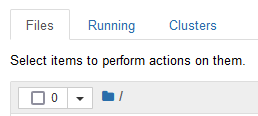
\includegraphics[width=0.4\textwidth]{img/Gamma3.PNG}
 \caption{Botón Running}
 \label{f:running}
\end{figure}

\begin{figure}[h]
 \centering
  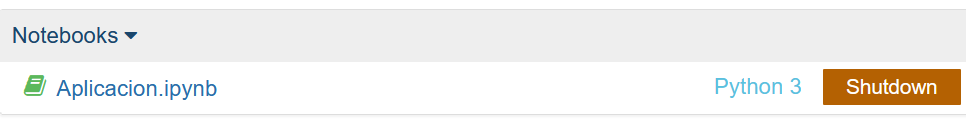
\includegraphics[width=1\textwidth]{img/Gamma4.PNG}
 \caption{Botón Shutdown}
 \label{f:shutdown}
\end{figure}


\bibliographystyle{plain}
\bibliography{bibliografiaAnexos}

\end{document}
